\documentclass[14pt,a4paper,report]{report}
\usepackage[a4paper, mag=1000, left=2.5cm, right=1cm, top=2cm, bottom=2cm, headsep=0.7cm, footskip=1cm]{geometry}
\usepackage[utf8]{inputenc}
\usepackage[english,russian]{babel}
\usepackage{indentfirst}
\usepackage[dvipsnames]{xcolor}
\usepackage[colorlinks]{hyperref}
\usepackage{listings} 
\usepackage{fancyhdr}
\usepackage{caption}
\usepackage{amsmath}
\usepackage{graphicx}
\usepackage{amsmath}
\usepackage{booktabs}
\usepackage{array}
\newcolumntype{P}[1]{>{\centering\arraybackslash}p{#1}}
\hypersetup{
	colorlinks = true,
	linkcolor  = black
}

\usepackage{titlesec}
\titleformat{\chapter}
{\Large\bfseries} % format
{}                % label
{0pt}             % sep
{\huge}           % before-code


\DeclareCaptionFont{white}{\color{white}} 

% Listing description
\usepackage{listings} 
\DeclareCaptionFormat{listing}{\colorbox{gray}{\parbox{\textwidth}{#1#2#3}}}
\captionsetup[lstlisting]{format=listing,labelfont=white,textfont=white}
\lstset{ 
	% Listing settings
	inputencoding = utf8,			
	extendedchars = \true, 
	keepspaces = true, 			  	 % Поддержка кириллицы и пробелов в комментариях
	language = C,            	 	 % Язык программирования (для подсветки)
	basicstyle = \small\sffamily, 	 % Размер и начертание шрифта для подсветки кода
	numbers = left,               	 % Где поставить нумерацию строк (слева\справа)
	numberstyle = \tiny,          	 % Размер шрифта для номеров строк
	stepnumber = 1,               	 % Размер шага между двумя номерами строк
	numbersep = 5pt,              	 % Как далеко отстоят номера строк от подсвечиваемого кода
	backgroundcolor = \color{white}, % Цвет фона подсветки - используем \usepackage{color}
	showspaces = false,           	 % Показывать или нет пробелы специальными отступами
	showstringspaces = false,    	 % Показывать или нет пробелы в строках
	showtabs = false,           	 % Показывать или нет табуляцию в строках
	frame = single,              	 % Рисовать рамку вокруг кода
	tabsize = 2,                  	 % Размер табуляции по умолчанию равен 2 пробелам
	captionpos = t,             	 % Позиция заголовка вверху [t] или внизу [b] 
	breaklines = true,           	 % Автоматически переносить строки (да\нет)
	breakatwhitespace = false,   	 % Переносить строки только если есть пробел
	escapeinside = {\%*}{*)}      	 % Если нужно добавить комментарии в коде
}

\begin{document}

\def\contentsname{Содержание}

% Titlepage
\begin{titlepage}
	\begin{center}
		\textsc{Санкт-Петербургский Политехнический 
			Университет Петра Великого\\[5mm]
			Кафедра компьютерных систем и программных технологий}
		
		\vfill
		
		\textbf{Отчёт по лабораторной работе №3.2\\[3mm]
			Курс: «Разработка экспертной системы с нуля»\\[41mm]
		}
	\end{center}
	
	\hfill
	\begin{minipage}{.4\textwidth}
		Выполнил студент:\\[2mm] 
		Ерниязов Т.Е.\\
		Группа: 13541/2\\[5mm]
		
		Проверил:\\[2mm] 
		Сазанов А.М.
	\end{minipage}
	\vfill
	\begin{center}
		Санкт-Петербург\\ \the\year\ г.
	\end{center}
\end{titlepage}

% Contents
\tableofcontents
\clearpage

\chapter{Лабораторная работа №3.2}

\section{Цель работы}

Научиться создавать экспертные системы с помощью конструктора Exsys CORVID.

\section{Программа работы}

\begin{enumerate}
	\item Разработайте экспертную систему для своего варианта индивидуального задания.
	\item Можно ли решить поставленную задачу проще без использования ЭС?
	\item В каких областях, по Вашему мнению, использование ЭС потенциально опасно (или вредно)?
\end{enumerate}

\clearpage

\section{Ход работы}

\subsection{Разработайте экспертную систему для своего варианта индивидуального задания}

\textbf{Тема 1.} Экспертная система по выбору оператора сотовой связи. Входные данные:

\begin{enumerate}
	\item зона уверенного приема сигнала
	\item стоимость роуминга
	\item предостовляемые услуги SMS, MMS, WAP
	\item тарифные планы
\end{enumerate}

Разработаем логическую схему работы требуемой экспертной системы. Система состоит из одного логического блока.

В экспертной системе реализовано 12 различных сценариев.

Пользователь выбирает нужные параметры, после чего на экране появляеться подходящий тариф.

Реализация логического блока:

\begin{figure}[h!]
	\centering
	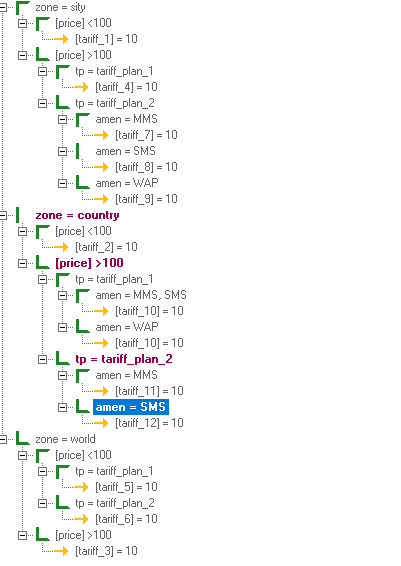
\includegraphics[scale = 0.90]{images/1.png}
	\caption{Реализация основного логического блока}
\end{figure}


Текст, выводимый на экран практически полностью определяется введенными переменными:

\begin{figure}[h!]
	\centering
	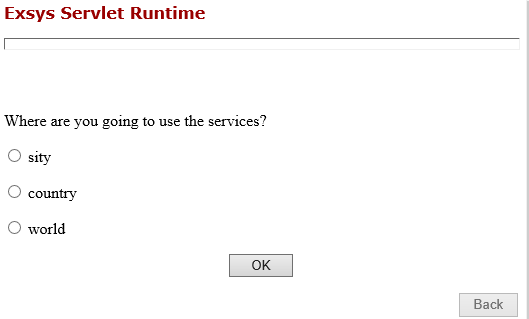
\includegraphics[scale = 0.85]{images/2.png}
	\caption{Определение зоны пользования}
\end{figure}


\begin{figure*}[h!]
	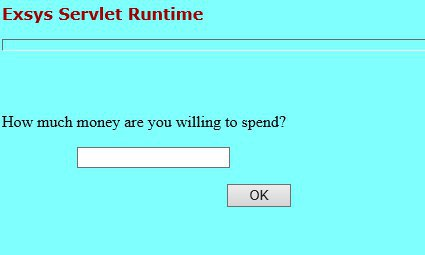
\includegraphics[width=.90\textwidth]{images/3.jpg}\hfill
	\caption{Ввод цены}
\end{figure*}

\clearpage
\begin{figure}[h!]
	\centering
	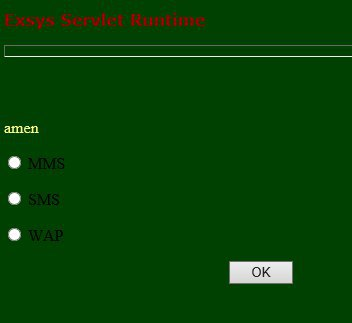
\includegraphics[scale = 0.80]{images/4.jpg}
	\caption{Выбор услуг}
\end{figure}

\begin{figure}[h!]
	\centering
	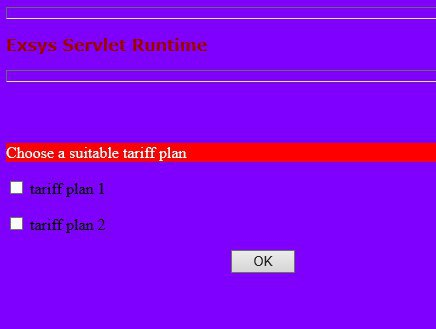
\includegraphics[scale = 0.70]{images/5.jpg}
	\caption{Выбор тарифного плана}
\end{figure}

Рассмотрим работу системы на примере этого сценария:

\begin{figure}[h!]
	\centering
	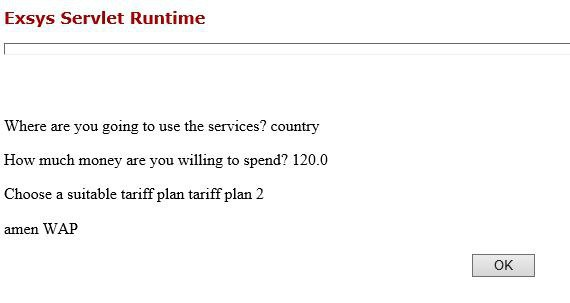
\includegraphics[scale = 0.90]{images/6.jpg}
	\caption{Если комплектация не укладывается в бюджет}
\end{figure}

\clearpage
\subsection{Можно ли решить поставленную задачу проще без использования ЭС?}

Да, можно. Самый легкий вариант в это области посоветоваться с консультантом. 

\subsection{В каких областях, по Вашему мнению, использование ЭС потенциально опасно (или вредно)?}

\begin{itemize}
	\item В областях, где накопленные знания быстро меняются или устаревают.
	\item В областях, где необходимо принятие незамедлительного решения, основанного на опыте и умении специалиста.
	\item В очень широких областях, где продолжительность диалога с пользователем стремится к бесконечности.
\end{itemize}

\section{Вывод}

В результате работы была успешно реализована ЭС для задачи выбора оператора сотовой связи. В ходе работы использовались различные виды переменных: статические списки и числовые переменные. Также видоизменен дизайн вывода для пользователя.



\section{Список литературы}

% \linebreak

\begin{flushleft}
	
[1] РАЗРАБОТКА ЭКСПЕРТНЫХ СИСТЕМ, О.А. ТАДЖИБАЕВА [Электронный ресурс]. — URL: \href{http://artlib.osu.ru/web/metod/655_20110711.pdf}{http://artlib.osu.ru/web/metod/655\_20110711.pdf} (дата обращения 21.10.2018). \linebreak

\end{flushleft}
	


\end{document}